\documentclass[aps,pre,twocolumn,superscriptaddress,floatfix,nofootinbib]{revtex4-2}

\usepackage{amsmath,amssymb}
\usepackage{graphicx}
\renewcommand{\thetable}{S\arabic{table}}
\renewcommand{\thefigure}{S\arabic{figure}}

\begin{document}

\title{Supplemental Material: Phase diagram of networks grown with triadic closure rules}

\author{Alexei Vazquez}
\email{alexei@nodeslinks.com}
\affiliation{Nodes \& Links Ltd, Salisbury House, Station Road, Cambridge, CB1 2LA, UK}

\date{\today}

\maketitle

\section{Per-triad rates}

Let every node spawn a newcomer at rate $\alpha_+$, which links to it, and every
open triad close at rate $\beta_+$ ($\beta_-=\alpha_-=0$). The number of nodes
grows as $n\propto e^{\alpha_+t}$, so node ages $\tau$, in units of
$1/\alpha_+$, are exponentially distributed, with density $e^{-\tau}$. In the
uncorrelated limit each neighbour of node $i$ has on average
$m=\langle k(k-1)\rangle/\langle k\rangle$ further neighbours, so $i$ is an
endpoint of about $k_im$ open triads (closed ones are negligible here), and
\begin{equation}
  \frac{dk}{d\tau}=1+xk,\qquad x=\frac{\beta_+m}{\alpha_+},
\end{equation}
and, with $k(0)=1$, $k(\tau)=(1+1/x)e^{x\tau}-1/x$. Averaging over ages,
\begin{equation}
  \langle k\rangle=\frac{2}{1-x},\qquad
  \langle k^2\rangle=\frac{(1+1/x)^2}{1-2x}-\frac{2(1+1/x)}{x(1-x)}+\frac1{x^2},
\end{equation}
and $P(k)\sim k^{-1-1/x}$. The second moment is finite only for $x<1/2$.
Self-consistency requires $m(x)=(\langle k^2\rangle-\langle k\rangle)/\langle k\rangle$,
which fixes $\beta_+/\alpha_+=x/m(x)$. This function vanishes at $x=0$ and at
$x=1/2$, where $m$ diverges, and has a maximum $\beta_+/\alpha_+=0.067$ at
$x=0.225$, where $\langle k\rangle=2.58$. Above it there is no stationary
density.

We simulated rule (w) with these rates, the closure probability per event
being $\beta_+W/(\alpha_+n+\beta_+W)$. For $\beta_+/\alpha_+\ge0.06$ the mean
degree runs away within $10^3$--$5\times10^4$ nodes. At $0.02$ and $0.04$ it
stays near $2.09$ and $2.23$ for a while. The plateau at $0.04$ corresponds to
an effective $u=1-2/\langle k\rangle\approx0.10$; the run condenses near
$n=10^6$, as in Sec.~VI of the main text, after which $W\sim n^{3/2}$, closures
outpace arrivals, and $\langle k\rangle$ reaches $2.67$ at $1.6\times10^6$ and
keeps rising.

\section{Data near the boundary and in the tree phase}

The tables and figure below give the data near the condensation boundary and in the tree
phase of rule (w) referred to in the main text. All runs use the code in the repository
cited there; the data files are \texttt{data/rev\_points.csv},
\texttt{data/rev\_brackets.csv} (\texttt{brackets.py}), and
\texttt{data/rev\_seeds.csv}, \texttt{data/rev\_traj.csv} and
\texttt{data/rev\_tree.csv} (\texttt{rev.py}); Fig.~S1 is drawn by \texttt{mkfigs.py}.

The cumulant in Table~S2, $U=1-\langle P_\triangle^4\rangle/(3\langle
P_\triangle^2\rangle^2)$, is $2/3$ for a narrow distribution. It stays at
$0.66$ in the condensed phase and dips at $0.76$ and $0.78$, where a few seeds
percolate and the distribution of $P_\triangle$ is broad and skewed. The scaled
variance $n\,{\rm var}(P_\triangle)$ peaks at $0.76$ at every size and grows as
$n^{0.55}$ between $10^4$ and $10^5$ and as $n^{0.94}$ between $10^5$ and
$10^6$.

The brackets of Table~S1 were also tested against the coordinates in which
deletion might act through density or through the rates per surviving node.
Neither collapses them. At $\langle k\rangle\approx3$ the boundary lies at
$0.73$ ($\Delta=1/2$, $\alpha_-=0$) and at $0.875$ ($\Delta=1$,
$\alpha_-/\alpha_+=0.3$), while at $\alpha_-/\alpha_+=0.5$ it lies at $0.89$ for
both $\Delta=1/2$ ($\langle k\rangle=2$) and $\Delta=1$ ($\langle
k\rangle=8/3$). At $\Delta=1$ the opening rate per net arrival at the boundary,
$\beta_-/(\alpha_+-\alpha_-)$, grows from $3.3$ to $62$, and the closure rate
$\beta_+/(\alpha_+-\alpha_-)$ from $4.3$ to $67$, between $\alpha_-/\alpha_+=0$
and $0.8$. A fit of $1-(\beta_-/\beta_+)_c$ linear in $1-\alpha_-/\alpha_+$ with
a free constant gives the constant $0.007$.

\begin{figure*}[t]
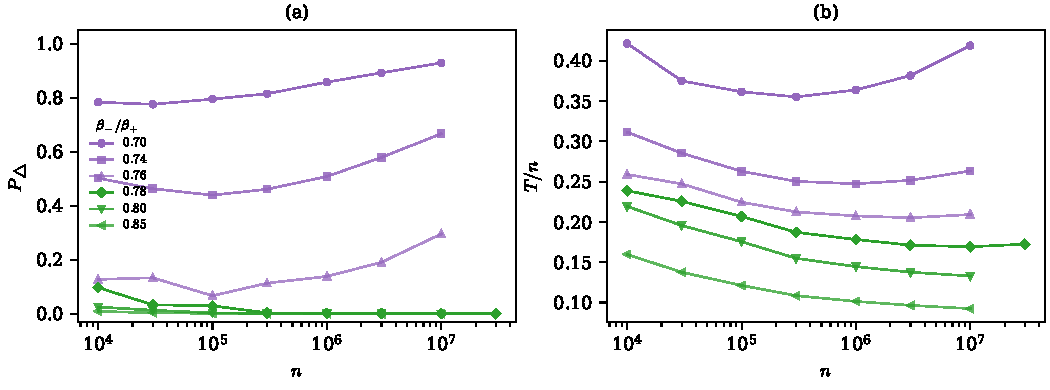
\includegraphics[width=\textwidth]{fig-traj.pdf}
\caption{Single trajectories to $n=10^7$ ($3\times10^7$ at $0.78$) near the boundary, rule (w) at
$\Delta=1$, $\alpha_-=0$, for the turnovers $\beta_-/\beta_+$ shown; each point
is the mean of two seeds, and smaller $n$ are earlier stages of the same runs.
Purple: turnovers that condense; green: turnovers that do not up to $10^7$.
(a) Order parameter $P_\triangle$. (b) Triangles per node $T/n$.}
\label{fig:traj}
\end{figure*}

\begin{table*}[t]
\caption{Brackets of the condensation boundary of rule (w). For each line of
net closure per arrival $\Delta$ and deletion $\alpha_-/\alpha_+$: the largest
condensed and the smallest dispersed turnover $\beta_-/\beta_+$, with the seed
mean of $P_\triangle$ at $n=10^5$ and $10^6$ and, in brackets, the number of
seeds. At $\Delta=1$, $\alpha_-/\alpha_+=0.9$ every point up to $0.95$ is
condensed.}
\label{tab:brackets}
\begin{ruledtabular}
\begin{tabular}{ccccccc}
$\Delta$ & $\alpha_-/\alpha_+$ & $\beta_-/\beta_+$ & $P_\triangle(10^5)$ & $P_\triangle(10^6)$ & $\beta_-/\beta_+$ & $P_\triangle(10^5)$, $P_\triangle(10^6)$\\
\hline
$1/2$ & $0$ & $0.72$ & $0.325$ (4) & $0.414$ (2) & $0.74$ & $0.151$ (4), $0.091$ (2)\\
$1/2$ & $0.5$ & $0.88$ & $0.591$ (4) & $0.706$ (2) & $0.9$ & $0.064$ (6), $0.001$ (3)\\
$1$ & $0$ & $0.76$ & $0.100$ (4) & $0.138$ (2) & $0.78$ & $0.021$ (4), $0.001$ (2)\\
$1$ & $0.1$ & $0.75$ & $0.604$ (2) & $0.706$ (1) & $0.8$ & $0.005$ (2), $0.001$ (1)\\
$1$ & $0.2$ & $0.8$ & $0.161$ (2) & $0.365$ (1) & $0.85$ & $0.003$ (2), $0.000$ (1)\\
$1$ & $0.3$ & $0.85$ & $0.008$ (2) & $0.039$ (1) & $0.9$ & $0.002$ (2), $0.000$ (1)\\
$1$ & $0.4$ & $0.85$ & $0.586$ (2) & $0.660$ (1) & $0.9$ & $0.002$ (2), $0.000$ (1)\\
$1$ & $0.5$ & $0.88$ & $0.206$ (4) & $0.442$ (2) & $0.9$ & $0.008$ (6), $0.001$ (3)\\
$1$ & $0.6$ & $0.9$ & $0.695$ (2) & $0.699$ (1) & $0.95$ & $0.002$ (2), $0.000$ (1)\\
$1$ & $0.7$ & $0.9$ & $0.931$ (2) & $0.979$ (1) & $0.95$ & $0.002$ (2), $0.000$ (1)\\
$1$ & $0.8$ & $0.9$ & $0.990$ (2) & $0.997$ (1) & $0.95$ & $0.007$ (2), $0.001$ (1)\\
\end{tabular}
\end{ruledtabular}
\end{table*}

\begin{table}[t]
\caption{Statistics of $P_\triangle$ over many seeds near the boundary,
$\Delta=1$, $\alpha_-=0$: mean and standard error, scaled variance
$n\,{\rm var}(P_\triangle)$ and cumulant $U=1-\langle P_\triangle^4\rangle/(3\langle P_\triangle^2\rangle^2)$,
with 64, 32 and 16 seeds at $n=10^4$, $10^5$ and $10^6$.}
\label{tab:seeds}
\begin{ruledtabular}
\begin{tabular}{ccccc}
$\beta_-/\beta_+$ & $n$ & $P_\triangle$ & $n\,{\rm var}(P_\triangle)$ & $U$\\
\hline
$0.70$ & $10^4$ & $0.7305\pm0.0063$ & $25.4$ & $0.66$\\
$0.70$ & $10^5$ & $0.7773\pm0.0036$ & $40.7$ & $0.67$\\
$0.70$ & $10^6$ & $0.8557\pm0.0028$ & $114.7$ & $0.67$\\
$0.72$ & $10^4$ & $0.6404\pm0.0081$ & $41.1$ & $0.65$\\
$0.72$ & $10^5$ & $0.6584\pm0.0076$ & $177.9$ & $0.66$\\
$0.72$ & $10^6$ & $0.7350\pm0.0063$ & $594.1$ & $0.67$\\
$0.74$ & $10^4$ & $0.4991\pm0.0119$ & $89.7$ & $0.63$\\
$0.74$ & $10^5$ & $0.4559\pm0.0093$ & $265.5$ & $0.65$\\
$0.74$ & $10^6$ & $0.5121\pm0.0082$ & $1014.7$ & $0.66$\\
$0.76$ & $10^4$ & $0.2756\pm0.0166$ & $173.2$ & $0.45$\\
$0.76$ & $10^5$ & $0.1402\pm0.0140$ & $606.8$ & $0.37$\\
$0.76$ & $10^6$ & $0.1369\pm0.0187$ & $5246.6$ & $0.41$\\
$0.78$ & $10^4$ & $0.0895\pm0.0085$ & $45.3$ & $-0.13$\\
$0.78$ & $10^5$ & $0.0095\pm0.0011$ & $4.0$ & $-0.05$\\
$0.78$ & $10^6$ & $0.0013\pm0.0002$ & $0.4$ & $0.30$\\
$0.80$ & $10^4$ & $0.0325\pm0.0024$ & $3.5$ & $0.13$\\
$0.80$ & $10^5$ & $0.0035\pm0.0002$ & $0.2$ & $0.44$\\
$0.80$ & $10^6$ & $0.0004\pm0.0000$ & $0.0$ & $0.58$\\
\end{tabular}
\end{ruledtabular}
\end{table}

\begin{table}[t]
\caption{Single trajectories at $\Delta=1$, $\alpha_-=0$, mean of two seeds:
$P_\triangle$, triangles per node $T/n$, largest degree $k_{\max}$, and the
share of all links that join two of the $1\%$ highest-degree nodes.}
\label{tab:traj}
\begin{ruledtabular}
\begin{tabular}{cccccc}
$\beta_-/\beta_+$ & $n$ & $P_\triangle$ & $T/n$ & $k_{\max}$ & top-$1\%$ links\\
\hline
$0.70$ & $10^5$ & $0.7951$ & $0.361$ & $107$ & $0.061$\\
$0.70$ & $10^6$ & $0.8580$ & $0.364$ & $208$ & $0.217$\\
$0.70$ & $10^7$ & $0.9293$ & $0.419$ & $462$ & $0.444$\\
$0.74$ & $10^5$ & $0.4392$ & $0.263$ & $92$ & $0.045$\\
$0.74$ & $10^6$ & $0.5084$ & $0.247$ & $174$ & $0.157$\\
$0.74$ & $10^7$ & $0.6669$ & $0.263$ & $374$ & $0.396$\\
$0.76$ & $10^5$ & $0.0667$ & $0.224$ & $91$ & $0.038$\\
$0.76$ & $10^6$ & $0.1384$ & $0.207$ & $163$ & $0.129$\\
$0.76$ & $10^7$ & $0.2954$ & $0.209$ & $326$ & $0.358$\\
$0.78$ & $10^5$ & $0.0294$ & $0.207$ & $82$ & $0.034$\\
$0.78$ & $10^6$ & $0.0014$ & $0.178$ & $144$ & $0.107$\\
$0.78$ & $10^7$ & $0.0003$ & $0.169$ & $279$ & $0.313$\\
$0.78$ & $3\times10^7$ & $0.0002$ & $0.172$ & $408$ & $0.419$\\
$0.80$ & $10^5$ & $0.0034$ & $0.175$ & $74$ & $0.027$\\
$0.80$ & $10^6$ & $0.0004$ & $0.144$ & $130$ & $0.076$\\
$0.80$ & $10^7$ & $0.0001$ & $0.133$ & $227$ & $0.231$\\
$0.85$ & $10^5$ & $0.0015$ & $0.121$ & $49$ & $0.013$\\
$0.85$ & $10^6$ & $0.0002$ & $0.101$ & $71$ & $0.025$\\
$0.85$ & $10^7$ & $0.0000$ & $0.092$ & $102$ & $0.049$\\
\end{tabular}
\end{ruledtabular}
\end{table}

\begin{table}[t]
\caption{Tree phase ($\beta_-=2\beta_+$) and tree transition ($\beta_-=\beta_+$)
at $\beta_+=\alpha_+$: range of the largest degree $k_{\max}$ and mean number
of triangles $T$ over four seeds.}
\label{tab:tree}
\begin{ruledtabular}
\begin{tabular}{ccccc}
$n$ & $k_{\max}$, $\beta_-=2\beta_+$ & $T$ & $k_{\max}$, $\beta_-=\beta_+$ & $T$\\
\hline
$10^4$ & $9$ & $0.2$ & $8--11$ & $74$\\
$10^5$ & $10--13$ & $1.8$ & $11--12$ & $174$\\
$10^6$ & $11--12$ & $1.2$ & $11--13$ & $796$\\
$10^7$ & $12--14$ & $1.2$ & $12--13$ & $2060$\\
\end{tabular}
\end{ruledtabular}
\end{table}

\end{document}
